% Options for packages loaded elsewhere
\PassOptionsToPackage{unicode}{hyperref}
\PassOptionsToPackage{hyphens}{url}
\PassOptionsToPackage{dvipsnames,svgnames,x11names}{xcolor}
%
\documentclass[
  super,
  review,
  3p]{elsarticle}

\usepackage{amsmath,amssymb}
\usepackage{iftex}
\ifPDFTeX
  \usepackage[T1]{fontenc}
  \usepackage[utf8]{inputenc}
  \usepackage{textcomp} % provide euro and other symbols
\else % if luatex or xetex
  \usepackage{unicode-math}
  \defaultfontfeatures{Scale=MatchLowercase}
  \defaultfontfeatures[\rmfamily]{Ligatures=TeX,Scale=1}
\fi
\usepackage{lmodern}
\ifPDFTeX\else  
    % xetex/luatex font selection
\fi
% Use upquote if available, for straight quotes in verbatim environments
\IfFileExists{upquote.sty}{\usepackage{upquote}}{}
\IfFileExists{microtype.sty}{% use microtype if available
  \usepackage[]{microtype}
  \UseMicrotypeSet[protrusion]{basicmath} % disable protrusion for tt fonts
}{}
\makeatletter
\@ifundefined{KOMAClassName}{% if non-KOMA class
  \IfFileExists{parskip.sty}{%
    \usepackage{parskip}
  }{% else
    \setlength{\parindent}{0pt}
    \setlength{\parskip}{6pt plus 2pt minus 1pt}}
}{% if KOMA class
  \KOMAoptions{parskip=half}}
\makeatother
\usepackage{xcolor}
\setlength{\emergencystretch}{3em} % prevent overfull lines
\setcounter{secnumdepth}{5}
% Make \paragraph and \subparagraph free-standing
\ifx\paragraph\undefined\else
  \let\oldparagraph\paragraph
  \renewcommand{\paragraph}[1]{\oldparagraph{#1}\mbox{}}
\fi
\ifx\subparagraph\undefined\else
  \let\oldsubparagraph\subparagraph
  \renewcommand{\subparagraph}[1]{\oldsubparagraph{#1}\mbox{}}
\fi


\providecommand{\tightlist}{%
  \setlength{\itemsep}{0pt}\setlength{\parskip}{0pt}}\usepackage{longtable,booktabs,array}
\usepackage{calc} % for calculating minipage widths
% Correct order of tables after \paragraph or \subparagraph
\usepackage{etoolbox}
\makeatletter
\patchcmd\longtable{\par}{\if@noskipsec\mbox{}\fi\par}{}{}
\makeatother
% Allow footnotes in longtable head/foot
\IfFileExists{footnotehyper.sty}{\usepackage{footnotehyper}}{\usepackage{footnote}}
\makesavenoteenv{longtable}
\usepackage{graphicx}
\makeatletter
\def\maxwidth{\ifdim\Gin@nat@width>\linewidth\linewidth\else\Gin@nat@width\fi}
\def\maxheight{\ifdim\Gin@nat@height>\textheight\textheight\else\Gin@nat@height\fi}
\makeatother
% Scale images if necessary, so that they will not overflow the page
% margins by default, and it is still possible to overwrite the defaults
% using explicit options in \includegraphics[width, height, ...]{}
\setkeys{Gin}{width=\maxwidth,height=\maxheight,keepaspectratio}
% Set default figure placement to htbp
\makeatletter
\def\fps@figure{htbp}
\makeatother

\makeatletter
\makeatother
\makeatletter
\makeatother
\makeatletter
\@ifpackageloaded{caption}{}{\usepackage{caption}}
\AtBeginDocument{%
\ifdefined\contentsname
  \renewcommand*\contentsname{Table of contents}
\else
  \newcommand\contentsname{Table of contents}
\fi
\ifdefined\listfigurename
  \renewcommand*\listfigurename{List of Figures}
\else
  \newcommand\listfigurename{List of Figures}
\fi
\ifdefined\listtablename
  \renewcommand*\listtablename{List of Tables}
\else
  \newcommand\listtablename{List of Tables}
\fi
\ifdefined\figurename
  \renewcommand*\figurename{Figure}
\else
  \newcommand\figurename{Figure}
\fi
\ifdefined\tablename
  \renewcommand*\tablename{Table}
\else
  \newcommand\tablename{Table}
\fi
}
\@ifpackageloaded{float}{}{\usepackage{float}}
\floatstyle{ruled}
\@ifundefined{c@chapter}{\newfloat{codelisting}{h}{lop}}{\newfloat{codelisting}{h}{lop}[chapter]}
\floatname{codelisting}{Listing}
\newcommand*\listoflistings{\listof{codelisting}{List of Listings}}
\makeatother
\makeatletter
\@ifpackageloaded{caption}{}{\usepackage{caption}}
\@ifpackageloaded{subcaption}{}{\usepackage{subcaption}}
\makeatother
\makeatletter
\@ifpackageloaded{tcolorbox}{}{\usepackage[skins,breakable]{tcolorbox}}
\makeatother
\makeatletter
\@ifundefined{shadecolor}{\definecolor{shadecolor}{rgb}{.97, .97, .97}}
\makeatother
\makeatletter
\makeatother
\makeatletter
\makeatother
\journal{People and Nature}
\ifLuaTeX
  \usepackage{selnolig}  % disable illegal ligatures
\fi
\usepackage[]{natbib}
\bibliographystyle{elsarticle-num}
\IfFileExists{bookmark.sty}{\usepackage{bookmark}}{\usepackage{hyperref}}
\IfFileExists{xurl.sty}{\usepackage{xurl}}{} % add URL line breaks if available
\urlstyle{same} % disable monospaced font for URLs
\hypersetup{
  pdftitle={Can we predict the predation pressure of owned domestic cats on all birds in the United States?},
  pdfauthor={Martin Philippe-Lesaffre},
  pdfkeywords={Domestic cat, Citizen science, Machine
learning, Management policies, Birds, Threats, Predation},
  colorlinks=true,
  linkcolor={blue},
  filecolor={Maroon},
  citecolor={Blue},
  urlcolor={Blue},
  pdfcreator={LaTeX via pandoc}}

\setlength{\parindent}{6pt}
\begin{document}

\begin{frontmatter}
\title{Can we predict the predation pressure of owned domestic cats on
all birds in the United States?}
\author[1,2]{Martin Philippe-Lesaffre%
%
}
 \ead{martin.philippe@universite-paris-saclay.fr} 

\affiliation[1]{organization={Université Paris-Saclay, CNRS,
AgroParisTech, Ecologie Systématique Evolution, IDEEV},addressline={12
rue
128},city={Gif-sur-Yvette},country={France},countrysep={,},postcode={91190},postcodesep={}}
\affiliation[2]{organization={https://orcid.org/0000-0002-1985-8758},,postcodesep={}}

\cortext[cor1]{Corresponding author}

        
\begin{abstract}
\begin{enumerate}
\def\labelenumi{\arabic{enumi}.}
\tightlist
\item
  Domestic cats (\emph{Felis catus}) have shared a common history with
  humans since their domestication 10,000 years ago and today they are
  one of the world's most widespread predatory mammals. Different
  populations of domestic cats around the world show a high degree of
  variability in terms of their autonomy from humans for feeding or
  moving about, with common descriptions ranging from owned domestic
  cats to feral domestic cats on the spectrum from the most dependent to
  the most autonomous with regard to humans. In this study, I quantified
  the potential ecological impact of owned domestic cats through
  predation, as the effects of these animals remain poorly understood at
  the large scale despite their abundance.
\item
  Distinguishing between owned and other domestic cats, I proposed a
  framework based on machine learning and citizen science data to
  predict the annual predation pressure on bird species per domestic cat
  considering traits, phylogeny and geographical distribution.
  Leveraging the Random Forest model and data from Mori et al.~(2019), I
  assessed the predation pressure for each native continental bird
  species of the United States.
\item
  Findings revealed that geographical distribution, phylogeny and traits
  influenced the predictive value of predation pressure, while a
  specific trait combination was also associated with high predation
  pressure. Furthermore, 35\% of species experienced high predation
  pressure from owned domestic cats regardless of the existing threats.
  The results are consistent with former empirical evidence of predation
  by domestic cats in the United States and highlight the urgency of
  understanding the ecological impact of domestic cats. By producing a
  quantitative value for predation pressure, the framework allows the
  development of more reliable models of species extinction risk,
  including for the effects of domestic cat predation, and thus the use
  of more specific management strategies to sensitive populations.
\item
  Although the study requires further refinement, the framework offers
  promising insights. With expanded citizen science protocols, it could
  help improve the extinction risk models and guide precise management
  strategies, which are crucial for mitigating the impact of domestic
  cats on native wildlife.
\end{enumerate}
\end{abstract}





\begin{keyword}
    Domestic cat \sep Citizen science \sep Machine
learning \sep Management policies \sep Birds, Threats \sep 
    Predation
\end{keyword}
\end{frontmatter}
    \ifdefined\Shaded\renewenvironment{Shaded}{\begin{tcolorbox}[borderline west={3pt}{0pt}{shadecolor}, boxrule=0pt, breakable, enhanced, interior hidden, sharp corners, frame hidden]}{\end{tcolorbox}}\fi

\hypertarget{introduction}{%
\section{\texorpdfstring{\textbf{Introduction}}{Introduction}}\label{introduction}}

Originating from the Near Eastern wildcat (Felis silvestris lybica), the
common house cat Felis catus was domesticated approximately 10,000 years
ago in the Fertile Crescent (Ottoni et al., 2017). Unlike many
domesticated species, cat populations exhibit significant variability in
terms of their level of independence from humans, particularly with
feeding, movement and reproduction, leading to a spectrum of domestic
cat populations, ranging from those under human ownership to completely
feral ones (Crowley et al., 2020). Today, stray, feral and free-ranging
domestic cats pose significant ecological threats as invasive species on
a global scale (Doherty et al., 2016; Medina et al., 2011; Oedin et al.,
2021). They have been linked to at least 26\% of bird, mammal and
reptile extinctions worldwide, particularly on islands (Doherty et al.,
2016), making their ecological impact on insular communities both acute
and uncontroversial (Bellard et al., 2017).

In continental ecosystems, particularly in North America, Eastern Europe
and Australia, domestic cats have been estimated to consume billions of
birds, mammals, amphibians and reptiles from hundreds of species
annually, thus prompting calls for broad-scale reductions in cat
populations (Blancher, 2013; Dauphine and Cooper, 2009; Doherty et al.,
2017; Doherty et al., 2015; Loss et al., 2013; Woods et al., 2003,
Woinarski et al., 2020). However, clear conclusions on the negative
impacts of domestic cats on native populations are still lacking due to
the limited number of studies investigating the ecological implications
of domestic cat predation on wildlife (van Heezik et al., 2010; Kosicki,
2021; Marzluff et al., 2016; Perkins et al., 2021). Within the spectrum
of domestic cat populations, owned domestic cats have garnered
increasing interest regarding their impact on native fauna, especially
in mainland regions (Woods et al., 2003; Brickner-Braun et al., 2007;
Loss and Marra, 2017; Mori et al., 2019; Mella-Mendez et al., 2022).
This interest stems from several factors, notably the global growth in
the population size, the range of owned domestic cats, the specificity
of managing owned domestic cats and the controversial nature of the
subject, even within the research community (Lynn et al., 2019).
Furthermore, countries have varying concerns about the impact of
domestic animals on fauna and, as a result, the implementation of
restrictive measures for owned domestic cats depends on the country and
can potentially face resistance from cat owners (Hall et al., 2016).

Recent approaches based on citizen science present a unique opportunity
to better quantify the impact of owned domestic cats worldwide,
especially due to the large scale of the data in terms of predation
events per identified species. Mori et al.~(2019) conducted a study on
145 domestic cats and recorded the number of predation events per
species per year. By contrast, most large-scale studies only produce a
binary classification of species -- 1 if the species was recorded as
prey and 0 if it was not -- or provide a unique predation pressure value
for all bird species. In parallel, recent studies have shown that
trophic relationships can be adequately predicted using species
characteristics and phylogeny in general (Caron et al., 2022;
Desjardins-Proulx et al., 2017; Gravel et al., 2013; Kopf et al., 2021;
O'Connor et al., 2020, Llewelyn et al., 2023) or for domestic cat
predation more specifically (Woinarski et al., 2017). Tree-based
algorithms are particularly effective at predicting these interactions,
not least because they can more easily deal with collinearity,
interactions between predictors, and response non-linearity, which are
suspected relationships when studying prey-predator relationships.
Therefore, the use of citizen science data for predation recordings
combined with tree-based algorithms could produce a more accurate
measure of predation pressure on species. It thus appears to be a unique
opportunity to provide more extensive and quantitative information on
the sensitivity of bird species on a large scale.

In this study, I compiled the traits, phylogeny, geographical range and
number of predation events recorded in the study of Mori et al.~(2019)
for all continental birds of Italy and North America. Based on this
information, I initially utilised the Italian birds as training data to
forecast the predation pressure of domestic cats in the United States by
computing Random Forest regression and then establishing connections
between traits, phylogeny and predation pressure. I focused on the
prediction of birds in the United States due to the substantial concerns
regarding the impact of owned domestic cats in the country, although the
available data lacks the necessary robustness, especially for birds
(Lepczyck et al., accepted). I also chose the United States, because it
has a similar co-evolutionary and biogeographical history to Italy. This
study therefore aimed to demonstrate that a citizen science approach
combined with supervised learning can facilitate the construction of
lists identifying vulnerable species across various scales, thus
enabling the development of more precise management strategies to
mitigate the impact of owned domestic cat predation on native fauna.

\hypertarget{methods}{%
\section{\texorpdfstring{\textbf{Methods}}{Methods}}\label{methods}}

All the analyses presented here were conducted using R Studio Version
2023.03.1+446 (R Core Team 2022)

\hypertarget{building-a-training-and-test-database-of-all-continental-birds-and-mammals-in-italy-and-the-united-states}{%
\subsection{Building a training and test database of all continental
birds and mammals in Italy and the United
States}\label{building-a-training-and-test-database-of-all-continental-birds-and-mammals-in-italy-and-the-united-states}}

I extracted all continental native birds of Italy and the United States
from the IUCN RedList database (2022) by compiling all species with a
native origin (`Native' for IUCN origin code) and currently present in
the country (`Extant' for IUCN presence code). The spatial distribution
of all native species was derived from BirdLife (2022), while the
geographic range of each species was defined as the number of 0.25° ×
0.25° latitude/longitude cells where the species was found in each
country divided by the total number of 0.25° × 0.25° latitude/longitude
cells in the country. Insular endemic species were removed. I thus
obtained a total of 337 species for Italy and 730 species for the United
States. For each selected species, I collected a set of morphological,
physiological and trophic traits. I based this selection on previous
evidence linking these traits to prey-predator relationships (Caron et
al., 2022; Desjardins-Proulx et al., 2017; Gravel et al., 2013; Kopf et
al., 2021; O'Connor et al., 2020) or linking them to domestic cat
predation in particular (Woinarski et al., 2017). I sourced seven traits
from two databases: body mass (continuous), tail length (continuous),
hand wing index (continuous), trophic niche (categorical: granivore,
vertivore, aquatic predator, invertivore, omnivore, nectarivore, aquatic
herbivore, terrestrial herbivore, frugivore, scavenger) and primary
lifestyle (categorical: insessorial, generalist, terrestrial, aerial,
aquatic) from the AVONET database (Tobias et al.~2022); and clutch size
(numeric) from Marino \& Bellard (2023). I obtained information about
species' habitat from the IUCN (2022) by adding eight dummy variables
for each main habitat (wetlands, shrubland, grassland, wetlands,
artificial/terrestrial, rocky, forest), where 0 indicates that the
species is absent from this habitat and 1 else. Using the two databases,
I removed all species with a geographical range of 0, leading to 303
bird species for Italy and 644 for the United States. The predation
pressure of Italian bird species was taken from Mori et al.~(2019) who
include several record events of predation based on 145 domestic cats
over the course of 1 year. I used the number of predation events per
year per cat per species as a standardised measure of predation
pressure. For each species in the United States, I additionally used the
Avian Conservation Assessment Database (ACAD) (Partners in Flight, 2021)
to extract four continental vulnerability factors (ordinal value between
1 and 5) based on Partners in Flight (PIF): population size, breeding
distribution, threats during breeding seasons and population trend.

\hypertarget{implementing-an-optimised-random-forest-to-predict-prey-predation-in-the-united-states-based-on-predation-pressure-on-italian-prey}{%
\subsection{Implementing an optimised Random Forest to predict prey
predation in the United States based on predation pressure on Italian
prey}\label{implementing-an-optimised-random-forest-to-predict-prey-predation-in-the-united-states-based-on-predation-pressure-on-italian-prey}}

To predict the predation pressure of birds in the United States, I built
a Random Forest regression using the Italian database as a training
dataset with the ranger R function of the ranger R package (Wright et
al., 2015). The number of predation events per year per cat was used as
a response variable and the seven traits, seven habitats and
geographical range as predictors. To deal with phylogenetic information
not included in the other previously compiled predictors, I added
phylogenetic eigenvector mapping (Guénard et al., 2013) to both
datasets. I extracted phylogenies for birds from VertLife.org and used
the MPSEM (Guénard and Legendre 2022), ape (Paradis and Schliep, 2019)
and phytools (Revell, 2012) R packages to calculate phylogenetic
eigenvectors for all species.

I optimised my Random Forest by adjusting the hyperparameters on the
training dataset. The optimisation was based on the minimisation of the
root mean square error (RMSE) of each species' out-of-bagging
prediction. I also provided the percentage of gain in terms of RMSE
compared with a default Random Forest regression, which was defined as
using the seven traits, seven habitats, geographical range as predictors
of the predation pressure computed with the default hyperparameters
provided by the ranger R function of the ranger R package (Wright et
al., 2015). I performed a cartesian grid search for the following seven
hyperparameters:

\begin{enumerate}
\def\labelenumi{\arabic{enumi}.}
\item
  Fraction of features to consider for splitting at each tree node
  (values = 0.05, 0.15, 0.25, 0.333, 0.4 or 0.6);
\item
  Number of data points allowed in a terminal (leaf) node (values = 1,
  3, 5, 10, 20, 30, 50, 75, 100);
\item
  Boolean value indicating whether sampling is done with replacement
  (\texttt{TRUE}) or without replacement (\texttt{FALSE});
\item
  Fraction of the total data used for each tree (values = 0.5, 0.6 or
  0.7);
\item
  Number of trees in the random forest (from 50 to 750 by step of 50);
\item
  Number of eigenvectors added to the dataset. I added the first 5, 10
  or 20 eigenvectors to the dataset to compute the Random Forest
  regression.
\item
  Weights assigned to different observations in the dataset, which give
  more importance to certain observations during training.
\end{enumerate}

I computed three weighting scenarios: firstly, with the same weight for
each species, then increasing the weight of the species with a strictly
positive response variable and then increasing the weight differently
for the most depredated species less the least depredated and again less
the non-depredated species. The three weighting scenarios were motivated
by the unbalanced dataset in which many species had no records of
predation. The hyperparameters producing the model with the lowest RMSE
were used to predict the predation event per year per cat using the
United States dataset as test data with the predicted R function of the
ranger R package (Wright et al., 2015).

\hypertarget{examining-optimised-random-forest-properties}{%
\subsection{Examining optimised Random Forest
properties}\label{examining-optimised-random-forest-properties}}

To assess the predictive power of this model for species predation, I
employed five key metrics of quality: R-squared (\(R^{2}\)), true
negative rate (TNR), true positive rate (TPR), F1-score and Matthews
correlation coefficient (MCC). These metrics are all based on the
comparison of 303 predicted values of predation pressure (i.e., the
value predicted for all species with the optimised Random Forest
regression) with the 303 observed values of predation pressure taken
from the Italian training dataset. TNR, TPR, F1-score and MCC are
designed for binary classifiers, which represented a challenge when
applied to my regression model. To address this issue, I added two
artificial binary outputs in the Italian dataset. Firstly, species with
a number of predation events per year per cat below 0.0069 (the lowest
value recorded in the database of Mori et al., 2019) were assigned a
predation value of 0 to indicate no predation, while species with
predation rates above this threshold were assigned a value of 1 to
denote predation. I similarly did the same for the predicted number of
predation events per year per cat computed using the Random Forest
regression. This binary classification allowed us to compute the five
metrics by evaluating the model's ability to predict species as either
prey or non-prey by comparing predation and predicted predation. It is
important to note that these metrics only evaluated the quality of the
regression to predict the species as prey or not, i.e., with a number of
predation events per year per cat above 0.0069. \(R^{2}\) is the only
metric that provided the quality of the model to predict the actual
number of predation events per year per cat. \(R^{2}\) was computed from
the linear regression of the predicted values of predation pressure as a
function of the observed values of predation pressure using the lm R
function of the stats R package. These metrics were used only for
post-hoc evaluation rather than for model optimisation.

To explore the global explanation of predictors and the contribution of
my Random Forest regression, I computed the Shapley-based feature
importance scores that correspond to the mean of the absolute value of
the feature contribution for each observation using the fastshap R
package (Greenwell et al., 2023). Results were displayed using the
shapviz and sv.importance R function of the fastshap R package
(Greenwell et al., 2023).

\hypertarget{exploring-prey-characteristics-of-italian-prey-and-predicted-prey-of-north-america}{%
\subsection{Exploring prey characteristics of Italian prey and predicted
prey of North
America}\label{exploring-prey-characteristics-of-italian-prey-and-predicted-prey-of-north-america}}

Firstly, I compared the results of the raw number of predation events
per year per cat for the Italian prey with the predicted number obtained
from the Random Forest by constructing two rarefaction curves. I then
used the predicted number of predation events per year per cat to build
a threshold of predation pressure. The first threshold is the threshold
of `no predation', corresponding to all species with several predation
events per year per cat under 0.0067, which is the lowest number
observed in the Mori et al.~(2019) database. Then I used the quantile R
function to extract the second quartile, median and third quartile of
the predicted number of predation events per year per cat in the
prediction obtained from the Italian training database for values above
the `no predation' threshold. I classified `weak predation' species
below the second quartile, `medium predation' species between the second
quartile and the median, `high predation' species between the median and
third quartile and `very high predation' species above the third
quartile. I then classified the species in the United States database
using the same value for each threshold. I built a functional space to
explore how traits were linked to predation pressure for birds in the
United States. Continuous traits were log-transformed using natural
logarithms when necessary to fit a normal distribution. To avoid
redundancy between traits, I initially analysed paired correlations
using Spearman's rank correlation coefficient (\(\rho\)) when comparing
two continuous traits with the cor R function, adjusted Cramér's V when
comparing two categorical traits using the cramerV R function of the
rcompanion R package (Mangiafico \& Mangiafico , 2017) and the \(R^{2}\)
of the linear regression between continuous and categorical traits
computed with the lm function of the stats R package. The uncorrelated
traits were selected to build a functional space using principal
component analysis with a varimax rotation computed with the PCAmix and
PCArot R function of the PCAmixdata R package (Chavet et al., 2014). I
selected the number of principal components based on the elbow method.
To compare the habitat types and vulnerability factor scores associated
with the lower or higher values of predicted predation pressure, I
firstly computed a linear regression with the predicted number of
predation events per year per cat as the response variable and habitat
or vulnerability factor score as the predictor using the aov R function
of the stats R package and then compared pairwise estimates with Tukey
honest significant differences using the TukeyHSD R function of the
stats R package. The predicted values of the number of predation events
per year per cat were transformed into their square root form using the
sqrt function to match normality, while the residuals were checked using
the R package DHARMa (Hartig, 2017).

To compare the predicted values of the number of predation events per
year per cat between species with empirical records of predation
extracted from Lepczyck et al.~(accepted) and those with no records, I
used a permutation test. I computed the median difference between the
two groups of species and then built 1,000 permutations with a random
permutation of species between groups using the sample R function. For
each of these 1,000 permutated datasets, I computed the median
difference between the two groups of species. The p-value was the number
of median differences of the permutated datasets above the median
difference measure in the original dataset divided by 1,000 (i.e.,
number of permutations)

\hypertarget{results}{%
\section{\texorpdfstring{\textbf{Results}}{Results}}\label{results}}

The raw number of predation events per year per cat extracted from Mori
et al.~(2019) ranges from 0 to 0.69, with 227 species with no records of
predation events and 76 with records (Fig. 1A). The mean value was 0.013
\(\pm\) 0.059 (hereafter, \(\pm\) indicates the standard deviation) for
all the continental birds of Italy and 0.053 \(\pm\) 0.11 if when
focusing on species with at least one recorded predation event in the
Mori et al.~(2019) database (i.e., 0.0067 number of predation events per
year per cat). The optimised Random Forest had a RMSE based on the
out-of-bagging prediction of 0.0030 (percentage gain compared with a
default Random Forest of 96\%). In terms of quality, the optimised
Random Forest regression had an \(R^{2}\) of 0.52, TNR of 0.93, TPR of
0.47, F1-score of 0.60 and MCC of 0.46. The predicted number of
predation events per year per cat ranged from 0.00035 to 0.14 in Italy
with a mean value of 0.016 \(\pm\) 0.022. Without species below 0.0069,
the mean predicted number of predation events per year per cat reached
0.029 \(\pm\) 0.024 (Fig. 1B). For species above the threshold of `low
predation' set at 0.0069, I obtained a first quartile or `medium
predation' threshold of 0.011, a median or `high predation' threshold of
0.020 and a third quartile or `very high predation' threshold of 0.042
(Fig. 1C). The absolute mean Shapley values of the optimised Random
Forest showed differences in terms of the importance of each predictor
to predict different values of predation pressure. Geographical range
was the most important predictor to predict predation pressure with
mean(\textbar SHAP value\textbar) = 0.0073 followed by hand wing index
with mean(\textbar SHAP value\textbar) = 0.0046 and the phylogenetic
information included in the two first eigenvectors with
mean(\textbar SHAP value\textbar) = 0.0034 and 0.0028 (Fig. 1C). In the
United States, the Random Forest regression produced a predicted number
of predation events per year per cat ranging from 0.00038 to 0.12 with a
mean value of 0.018 \(\pm\) 0.017. Using the threshold computing from
the Italian dataset, I obtained 231 species with `no predation', 70
species with `low predation', 115 species with `medium predation', 170
with `high predation' and 58 species with `very high predation' (Figs 2A
\& 2B). Primary lifestyle and trophic niche were highly correlated with
the hand wing index (\(R^{2}\) = 0.7 and \(R^{2}\) = 0.68) (Supp. Fig.
1). Similarly, tail length was highly correlated with body mass
(\(\rho\) = 0.68). Clutch size displayed no correlation coefficient
above 0.5. I also noticed that the first and the second eigenvector were
correlated with \(\rho\) = 0.59 and the first eigenvector was highly
correlated with trophic niche (\(R^{2}\) = 0.72), body mass (\(\rho\) =
0.74) and hand wing index (\(\rho\) = 0.69). Consequently, the
functional space was built using body mass, clutch size and hand wing
index. The first principal component (PC1) of the functional space
explained 45\% of the variance and the second (PC2) explained 39\% (Fig.
2C). Overall, 85\% of the variance of body mass and 50\% of the variance
of hand wing index were explained by PC1, while 92\% of the variance of
clutch size and 25\% of the variance of hand wing index were explained
by PC2 (Fig. 2C). Species with `very high predation' and `high
predation' classifications were more clustered at negative values of
PC1, whereas species with `no predation' classifications were more
clustered at positive values. Species with `medium predation' and `low
classification' seemed distributed along the PC1 (Fig. 2D). The
distribution of species along PC2 was less evident, as only species with
a `very high predation' classification were clustered around null values
of PC2 (Fig. 2E). The habitat most associated with higher predation
pressure was shrubland, which displayed significantly higher predictions
compared with all other habitats (Fig. 3), followed by
artificial/terrestrial and forest, which displayed significantly lower
predictions than shrubland but significantly higher predictions than the
other habitats. Grassland, rocky and wetland were the habitats showing
the lowest prediction of predation pressure. Predation pressures were
equally distributed between species with different levels of threats
fore one PIF continental vulnerability factor, namely population trend
(Fig. 4). For the population size factor, the least threatened species
(i.e., score of 1) were significantly predicted with more predation
pressure than all other scores (Fig. 4). Similarly, species with a score
of 2 were significantly predicted with more predation pressure than
species with a score of 3, 4 and 5. No differences were observed between
species with a score of 3, 4 or 5. A similar pattern was observed for
the threats during breeding factor, except for species with a score of
5, which were predated as much as those with a score of 2, 3 or 4. For
breeding distribution factor, I observed a weaker effect with only the
species with a score of 1 being predicted with more predation pressure
than the species with a score of 4 or 5. When comparing these results
with the known prey species taken from the North American database of
Lepczyk et al.~(accepted), I observed that the predicted number of
predation events per year per cat was significantly higher for species
already known as prey compared with species with no records of predation
(mean difference permutation test, p-value = 0) (Fig. 5A). More
precisely, the median value of predation pressure for species with
empirical records was 0,020 against 0.0079 for species with no records.
Similarly, of the 421 species with no empirical records of predation,
194 were assigned to `no predation' by the Random Forest regression
(46\% of species), whereas 37 of the 223 species with empirical records
of predation were assigned to `no predation' (17\%) (Fig. 5B). For the
species with empirical records, 119 species had a `high' or `very high
predation' pressure (28\%) compared with 109 species for those with no
records (49\%) (Fig. 5B).

\hypertarget{discussion}{%
\section{\texorpdfstring{\textbf{Discussion}}{Discussion}}\label{discussion}}

In this study, the utilisation of citizen science data permitted the
construction of a Random Forest regression model to predict species
predation pressure based on traits, phylogeny and geographical range
with notable accuracy. My findings highlighted the significance of
geographical range, phylogeny and hand wing index as primary predictors
that influence the number of predation events per year per cat, thus
serving as a proxy for predation pressure.

Applying this model to assess the predation pressure exerted by domestic
cats on bird species in the United States, my analysis of 644 species
revealed that a substantial 35\% of species were categorised as `high
predation' or `very high predation'. Furthermore, species with higher
predicted predation pressure exhibited specific trait combinations, thus
emphasising the nuanced nature of predation vulnerability. In terms of
habitat, birds found in shrubland, forest and artificial/terrestrial
habitats displayed heightened sensitivity compared with other species,
thus underscoring the impact of habitat preference on predation
pressure.

Concerns about conservation status may thus arise, especially for
species facing high predation pressure from domestic cats because
species with high threat scores were also likely to experience high
predation pressure, as indicated by the population trend factor in the
ACAD database for which the score (from 1 to 5) did not influence
predation pressure. However, for the other three factors, I also found
that species with lower vulnerability scores faced lower predation. It
would therefore seem that the domestic cat would tend to predate less
vulnerable species on a continental scale, but it should be remembered
that these factors do not take into account the more local vulnerability
of the populations that the cat could impact (van Heezik et al., 2010).

However, the reliability of the predicted predation pressure reported in
this article faces several challenges due to the absence of equivalent
studies akin to that of Mori et al.~(2019), which could provide robust
evidence. Nevertheless, my findings were corroborated by Lepczyk et
al.~(accepted), who recently compiled a comprehensive global dataset of
domestic cat predation events. A positive trend emerged when comparing
my results with existing empirical records, indicating higher predation
pressure for species with documented records. Importantly, my predictive
approach and empirical records provided complementary insights. While
species with existing empirical records generally showed higher
predation pressure, some exhibited surprisingly low predation pressure,
suggesting potential biases such as taxonomic and database limitations
or imperfections in the Random Forest model due to the scarcity of
predation event records.

Most studies examining the impact of domestic cats on native species
focus on predation at broad taxonomic levels (Loss et al., 2013), local
scales (Mella-Mendez et al., 2022) or binary classifications (prey or
non-prey; see Lepczyk et al., accepted). My framework, however, offered
a unique opportunity by quantifying predation pressure at a fine
taxonomic resolution and high spatial accuracy. By moving beyond binary
classifications, we differentiated species with weak or low predation
pressure, thus providing a more nuanced understanding of the impact of
domestic cats on native fauna. While my model's exact predictions
exhibited some uncertainties, the categorical classifications and
rankings presented more robust outcomes.

Looking to the future with enhanced citizen science databases that offer
broader sampling coverage, this framework could be significantly
improved. In scenarios with highly robust Random Forest regression
models, the predicted number of predation events per year per cat could
be used directly to explore population extinction risks based on species
density and domestic cat density. Adjustments for correction factors
that consider that only a portion of prey items are brought home
(Piontek et al., 2021) are essential for accurate predictions. My
framework is notably biased towards owned domestic cats and their prey
brought home, thus potentially overlooking highly predated species not
brought home such as larger prey. Additionally, the extension of the
results to semi-owned or feral domestic cats should be considered with
caution. Finally, it is crucial to acknowledge that while my framework
quantifies the impact of owned domestic cats through direct predation
alone, other mechanisms such as disease transmission, hybridisation and
sub-lethal effects can also impact native fauna (Loss and Marra, 2017).
Understanding these multifaceted dynamics is vital for the development
of comprehensive conservation and management strategies.

\hypertarget{references}{%
\section{\texorpdfstring{\textbf{References}}{References}}\label{references}}

Bellard, C., Rysman, J.-F., Leroy, B., Claud, C., Mace, G.M. (2017). A
global picture of biological invasion threat on islands. Nature Ecology
and Evolution 1: 1862--1869. https://doi.org/10.1038/s41559-017-0365-6.

Blancher P (2013) Estimated number of birds killed by house cats (Felis
catus) in Canada. Avian Conserv Ecol 8:3.
http://dx.doi.org/10.5751/ACE-00557-080203.

BirdLife International, \& Handbook of the Birds of the World. (2022).
Bird species distribution maps of the world.
http://datazone.birdlife.org/species/requestdi

Brickner-Braun, I., Geffen, E. L. I., \& Yom-Tov, Y. (2007). The
domestic cat as a predator of Israeli wildlife. Israel Journal of
Ecology \& Evolution, 53(2), 129-142.
https://doi.org/10.1560/IJEE.53.2.129.

Caron, D., Maiorano, L., Thuiller, W., \& Pollock, L. J. (2022).
Addressing the Eltonian shortfall with trait‐based interaction models.
Ecology Letters 25:, 889-89. https://doi.org/10.1111/ele.13966.

Chavent, M., Kuentz-Simonet, V., Labenne, A., \& Saracco, J. (2014).
Multivariate analysis of mixed data: The R package PCAmixdata. arXiv
preprint arXiv:1411.4911. https://doi.org/10.48550/arXiv.1411.4911.

Crowley, S. L., Cecchetti, M., \& McDonald, R. A. (2020). Our wild
companions: Domestic cats in the Anthropocene. Trends in Ecology \&
Evolution, 35(6), 477-483. https://doi.org/10.1016/j.tree.2020.01.008.

Dauphiné, N. I. C. O., \& Cooper, R. J. (2009, October). Impacts of
free-ranging domestic cats (Felis catus) on birds in the United States:
a review of recent research with conservation and management
recommendations. In Proceedings of the fourth international partners in
flight conference: tundra to tropics (Vol. 205).

Desjardins-Proulx, P., Laigle, I., Poisot, T., \& Gravel, D. (2017).
Ecological interactions and the Netflix problem. PeerJ, 5, e3644.
https://doi.org/10.7717/peerj.3644.

Doherty, T. S., Dickman, C. R., Johnson, C. N., Legge, S. M., Ritchie,
E. G., \& Woinarski, J. C. (2017). Impacts and management of feral cats
Felis catus in Australia. Mammal Review, 47(2), 83-97.
https://doi.org/10.1111/mam.12080.

Doherty, T. S., Glen, A. S., Nimmo, D. G., Ritchie, E. G., \& Dickman,
C. R. (2016). Invasive predators and global biodiversity loss.
Proceedings of the National Academy of Sciences, 113(40), 11261-11265.
https://doi.org/10.1073/pnas.1602480113.

Doherty, T. S., Davis, R. A., van Etten, E. J., Algar, D., Collier, N.,
Dickman, C. R., \ldots{} \& Robinson, S. (2015). A continental‐scale
analysis of feral cat diet in Australia. Journal of Biogeography, 42(5),
964-975. https://doi.org/10.1111/jbi.12469.

Hall, C. M., Adams, N. A., Bradley, J. S., Bryant, K. A., Davis, A. A.,
Dickman, C. R., et al.~(2016). Community attitudes and practices of
urban residents regarding predation by pet cats on wildlife: an
international comparison. PLoS ONE 11:e0151962.
https://doi.org/10.1371/journal.pone.0151962.

Hartig, Florian, and Maintainer Florian Hartig. ``Package `DHARMa'.'' R
package (2017). Gravel, D., Poisot, T., Albouy, C., Velez, L., \&
Mouillot, D. (2013). Inferring food web structure from predator--prey
body size relationships. Methods in Ecology and Evolution 4: 1083-1090.
https://doi.org/10.1111/2041-210X.12103.

Greenwell B (2023). fastshap: Fast Approximate Shapley Values.
https://github.com/bgreenwell/fastshap,
https://bgreenwell.github.io/fastshap/.

Guénard, G., \& Legendre, P. (2022). Hierarchical clustering with
contiguity constraint in R. Journal of Statistical Software, 103, 1-26.
https://doi.org/10.18637/jss.v103.i07.

Guénard, G., Legendre, P., \& Peres‐Neto, P. (2013). Phylogenetic
eigenvector maps: a framework to model and predict species traits.
Methods in Ecology and Evolution, 4(12), 1120-1131.
https://doi.org/10.1111/2041-210X.12111. IUCN. (2022). The IUCN Red List
of Threatened Species. iucnredlist.org.

Kopf, R. K., Yen, J. D., Nimmo, D. G., Brosse, S., \& Villéger, S.
(2021). Global patterns and predictors of trophic position, body size
and jaw size in fishes. Global Ecology and Biogeography, 30(2), 414-428.
https://doi.org/10.1111/geb.13227.

Kosicki, J., 2021. The impact of feral domestic cats on native bird
populations. Predictive modelling approach on a country scale.
Ecological Complexity. https://doi.org/10.1016/j.ecocom.2021.100964

Lepczyk C. A., Fantle-Lepczyk J. E., Dunham K., Bonnaud E., Lindner J.,
Doherty T.S., Woinarski J.C. Z. A. (accepted). Global Synthesis and
Assessment of Free-ranging Domestic Cat Diet. Nature Communications, in
press.

Llewelyn, J., Strona, G., Dickman, C. R., Greenville, A. C., Wardle, G.
M., Lee, M. S., \ldots{} \& Bradshaw, C. J. (2023). Predicting
predator--prey interactions in terrestrial endotherms using random
forest. Ecography, e06619. https://doi.org/10.1111/ecog.06619 Loss, S.
R., \& Marra, P. P. (2017). Population impacts of free‐ranging domestic
cats on mainland vertebrates. Frontiers in Ecology and the Environment
15: 502-509. https://doi.org/10.1002/fee.1633.

Loss, S. R., Will, T., \& Marra, P. P. (2013). The impact of
free-ranging domestic cats on wildlife of the United States. Nature
communications, 4(1), 1-8. https://doi.org/10.1038/ncomms2380.

Lynn, W. S., Santiago‐Ávila, F., Lindenmayer, J., Hadidian, J., Wallach,
A., \& King, B. J. (2019). A moral panic over cats. Conservation Biology
33: 769-776. https://doi.org/10.1111/cobi.13346.

Mangiafico, S., \& Mangiafico, M. S. (2017). Package `rcompanion'. Cran
Repos, 20, 1-71.

Marino, C., \& Bellard, C. (2023). When origin, reproduction ability and
diet define the role of birds in invasions. Proceedings of the Royal
Society B, 290(1995), 20230196. https://doi.org/10.1098/rspb.2023.0196.

Marzluff, J.M., Clucas, B., Oleyar, M.D., DeLap, J., 2016. The causal
response of avian communities to suburban development: a
quasi-experimental, longitudinal study. Urban Ecosyst 19, 1597--1621.
https://doi.org/10.1007/s11252-015-0483-3

Medina, F.M., Bonnaud, E., Vidal, E., Tershy, B.R., Zavaleta, E.S., Josh
Donlan, C., Keitt, B.S., Le Corre, M., Horwath, S.V., Nogales, M.
(2011). A global review of the impacts of invasive cats on island
endangered vertebrates. Global Change Biology 17: 3503--3510.
https://doi.org/10.1111/j.1365-2486.2011.02464.x.

Mella-Mendez, I., Flores-Peredo, R., Amaya-Espinel, J. D., Bolivar-Cime,
B., Mac Swiney G, M. C., \& Martínez, A. J. (2022). Predation of
wildlife by domestic cats in a Neotropical city: a multi-factor issue.
Biological Invasions, 24(5), 1539-1551.
https://doi.org/10.1007/s10530-022-02734-5.

Mori, E., Menchetti, M., Camporesi, A., Cavigioli, L., Tabarelli de
Fatis, K., \& Girardello, M. (2019). License to kill? Domestic cats
affect a wide range of native fauna in a highly biodiverse Mediterranean
country. Frontiers in Ecology and Evolution, 7, 477.
https://doi.org/10.3389/fevo.2019.00477.

O'Connor, L. M., Pollock, L. J., Braga, J., Ficetola, G. F., Maiorano,
L., Martinez‐Almoyna, C., \ldots{} \& Thuiller, W. (2020). Unveiling the
food webs of tetrapods across Europe through the prism of the Eltonian
niche. Journal of Biogeography 47: 181-192.
https://doi.org/10.1111/jbi.13773.

Oedin, M., Brescia, F., Millon, A., Murphy, B. P., Palmas, P.,
Woinarski, J. C., \& Vidal, E. (2021). Cats Felis catus as a threat to
bats worldwide: a review of the evidence. Mammal Review, 51(3), 323-337.
https://doi.org/10.1111/mam.12240. Ottoni, C., Van Neer, W., De Cupere,
B., Daligault, J., Guimaraes, S., Peters, J., \ldots{} \& Geigl, E. M.
(2017). The palaeogenetics of cat dispersal in the ancient world. Nature
Ecology \& Evolution, 1(7), 1-7.
https://doi.org/10.1038/s41559-017-0139.

Paradis, E., \& Schliep, K. (2019). ape 5.0: an environment for modern
phylogenetics and evolutionary analyses in R. Bioinformatics, 35(3),
526-528. https://doi.org/10.1093/bioinformatics/bty633.

Partners in Flight. 2021. Avian Conservation Assessment Database,
version 2021. Available at http://pif.birdconservancy.org/ACAD. Accessed
on 2023

Perkins, G.C., Martin, A.E., Smith, A.C., Fahrig, L., 2021. Weak Effects
of Owned Outdoor Cat Density on Urban Bird Richness and Abundance. Land
10, 507. https://doi.org/10.3390/land10050507

Piontek, A. M., Wojtylak-Jurkiewicz, E., Schmidt, K., Gajda, A., Lesiak,
M., \& Wierzbowska, I. A. (2021). Analysis of cat diet across an
urbanisation gradient. Urban Ecosystems, 24(1), 59-69.
https://doi.org/10.1007/s11252-020-01017-y.

R Core Team (2022). R: A language and environment for statistical
computing. R. Foundation for Statistical Computing, Vienna, Austria. URL
https://www.R-project.org/.

Revell, L. J. (2012). phytools: an R package for phylogenetic
comparative biology (and other things). Methods in ecology and
evolution, (2), 217-223.
https://doi.org/10.1111/j.2041-210X.2011.00169.x.

van Heezik, Y., Smyth, A., Adams, A., Gordon, J., 2010. Do domestic cats
impose an unsustainable harvest on urban bird populations? Biological
Conservation 143, 121--130. https://doi.org/10.1016/j.biocon.2009.09.013

Woods, M., McDonald, R. A., \& Harris, S. (2003). Predation of wildlife
by domestic cats Felis catus in Great Britain. Mammal review, 33(2),
174-188. https://doi.org/10.1046/j.1365-2907.2003.00017.x.

Woinarski, J. C. Z., Legge, S. M., Woolley, L. A., Palmer, R., Dickman,
C. R., Augusteyn, J., \ldots{} \& Murphy, B. P. (2020). Predation by
introduced cats Felis catus on Australian frogs: compilation of species
records and estimation of numbers killed. Wildlife Research, 47(8),
580-588. https://doi.org/10.1071/WR19182.

Woinarski, J. C. Z., Woolley, L. A., Garnett, S. T., Legge, S. M.,
Murphy, B. P., Lawes, M. J., \ldots{} \& Paton, D. (2017). Compilation
and traits of Australian bird species killed by cats. Biological
Conservation 216: 1-9. https://doi.org/10.1016/j.biocon.2017.09.017.

Wright, M. N., \& Ziegler, A. (2015). ranger: A fast implementation of
random forests for high dimensional data in C++ and R. arXiv preprint
arXiv:1508.04409. https://doi.org/10.48550/arXiv.1508.04409.**

\hypertarget{figures}{%
\section{\texorpdfstring{\textbf{Figures}}{Figures}}\label{figures}}

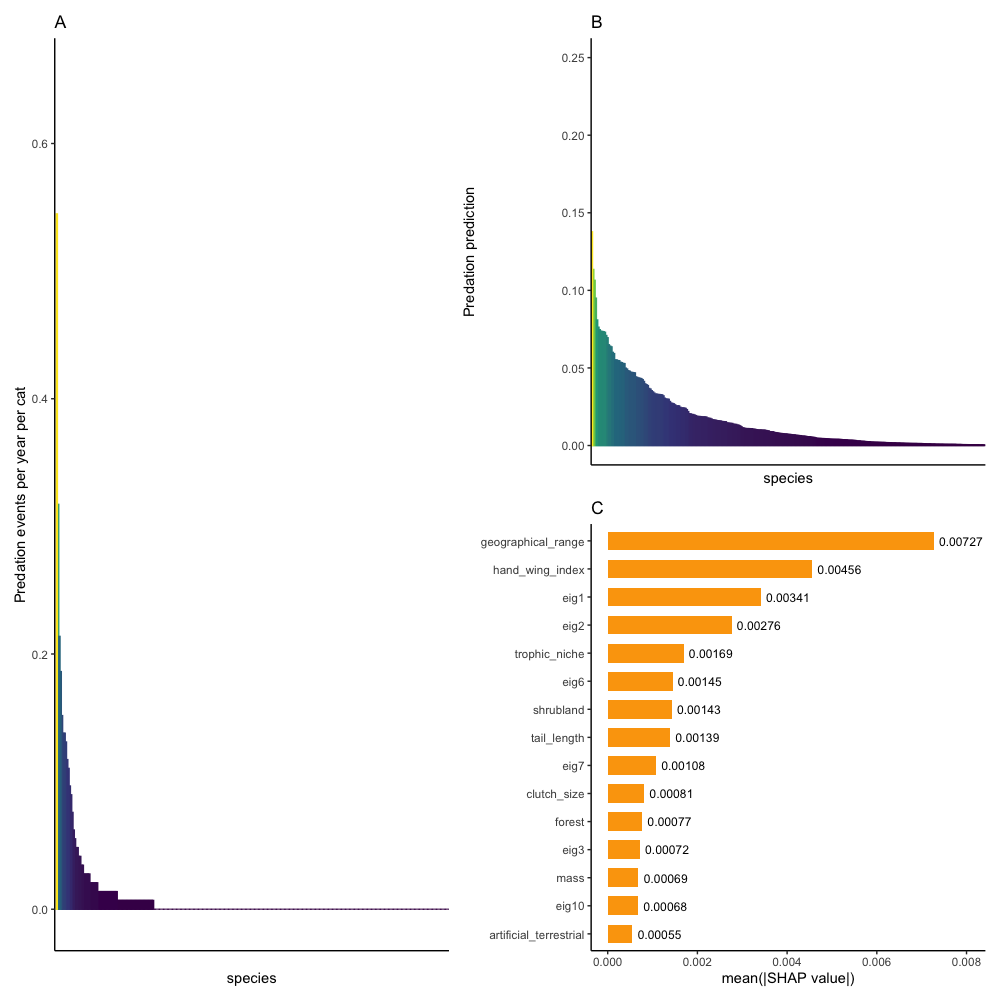
\includegraphics{Figure1.png} \textbf{Figure 1. Characteristics of the
Random Forest regression computed using data from Mori et al.~(2019) on
the predation pressure of domestic cats on native continental birds in
Italy.} Panel A depicts the species rarefaction curve generated from the
predation events recorded by 145 domestic cats over the course of 1
year, encompassing all native Italian birds. Panel B shows the species
rarefaction curve derived from the Random Forest regression that
predicts predation pressure. The model employs predation events per year
per cat per species as the response variable and considers traits,
phylogeny and geographical range as predictors, trained using the same
dataset. Panel C presents Shapley-based feature importance scores,
indicating the most influential predictors in the Random Forest
regression. These scores are based on the mean of the absolute value of
the feature contribution for each observation.

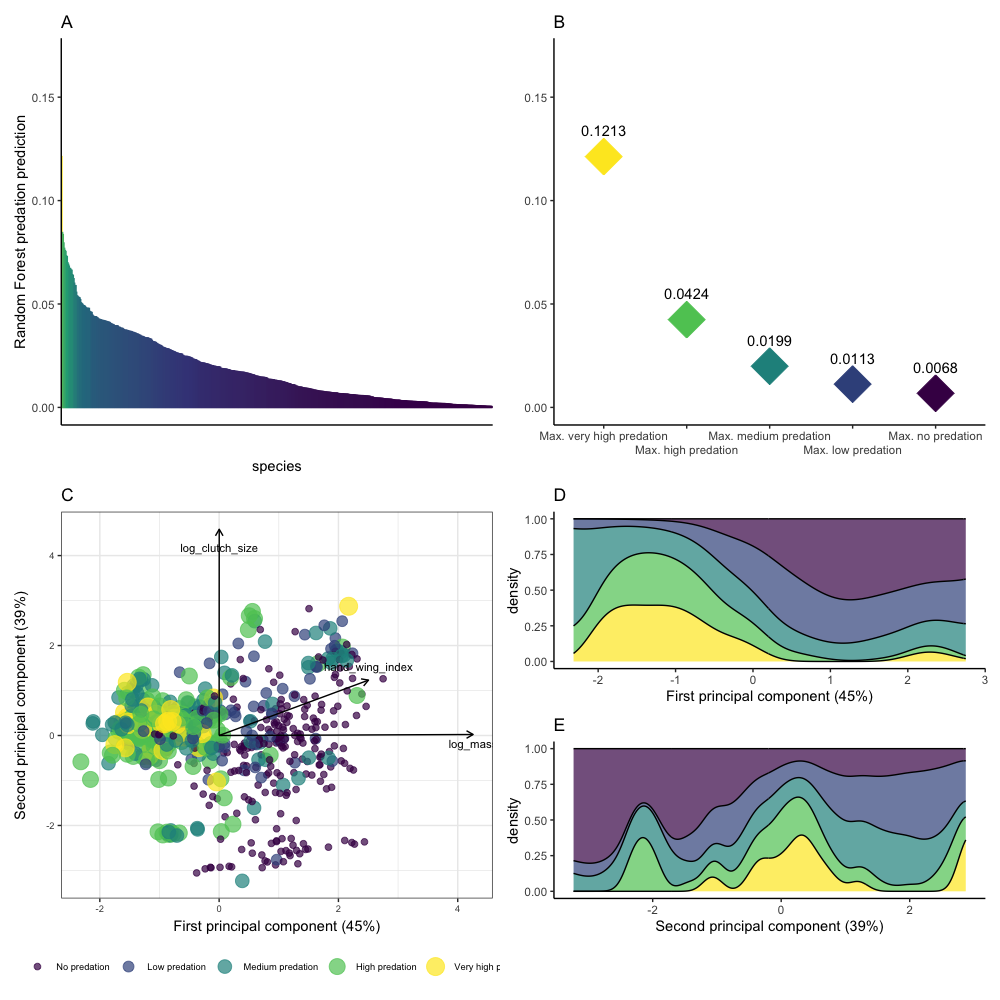
\includegraphics{Figure2.png} \textbf{Figure 2. Overview of the results
of the Random Forest regression for predicting domestic cat predation
pressure on all native continental birds in the United States and
associated traits.} Panel A displays the species rarefaction curve,
generated from the predation pressure predicted by the Random Forest
regression. The model employs predation events per year per cat per
species as the response variable, with traits, phylogeny and
geographical range as predictors, trained using the Italian data. Panel
B illustrates the maximum predicted predation events per year per cat
for each predation pressure classification. Panel C presents the
functional space constructed using three weakly correlated traits of all
native continental birds in the United States. Each point represents a
species, with the size proportional to predation pressure. Panels D and
E depict the distribution proportion of species across predation
pressure classifications along the first and second principal
components, which provides insights into the relationship between traits
and predation pressure.

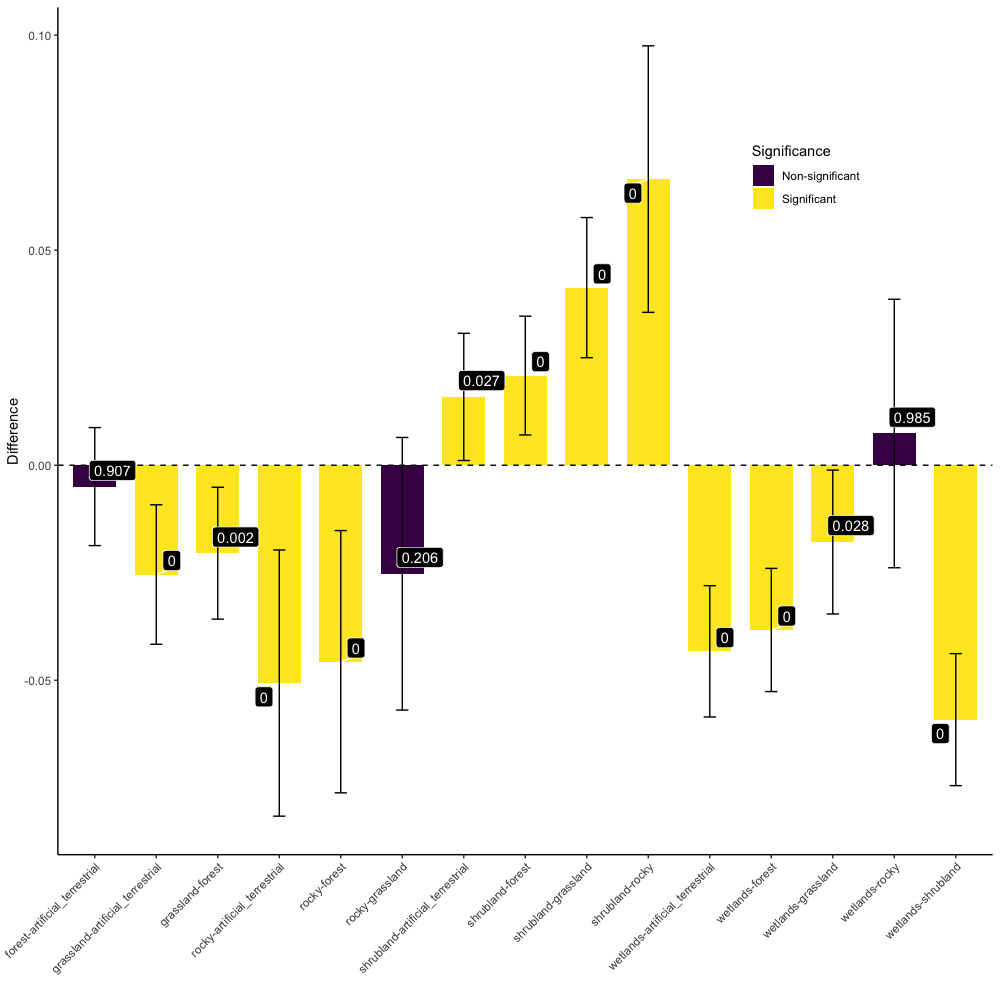
\includegraphics{Figure3.png} \textbf{Figure 3. Comparison of predicted
predation pressure of owned domestic cats across habitats for all native
continental birds in the United States.} Each bar in the figure
represents the difference between the means of two different habitats.
The accompanying bracket shows the 95\% confidence interval based on the
Tukey honest significant differences of the mean difference between the
habitats. The corresponding p-value, which indicates the statistical
significance of the observed differences, is provided in white font.

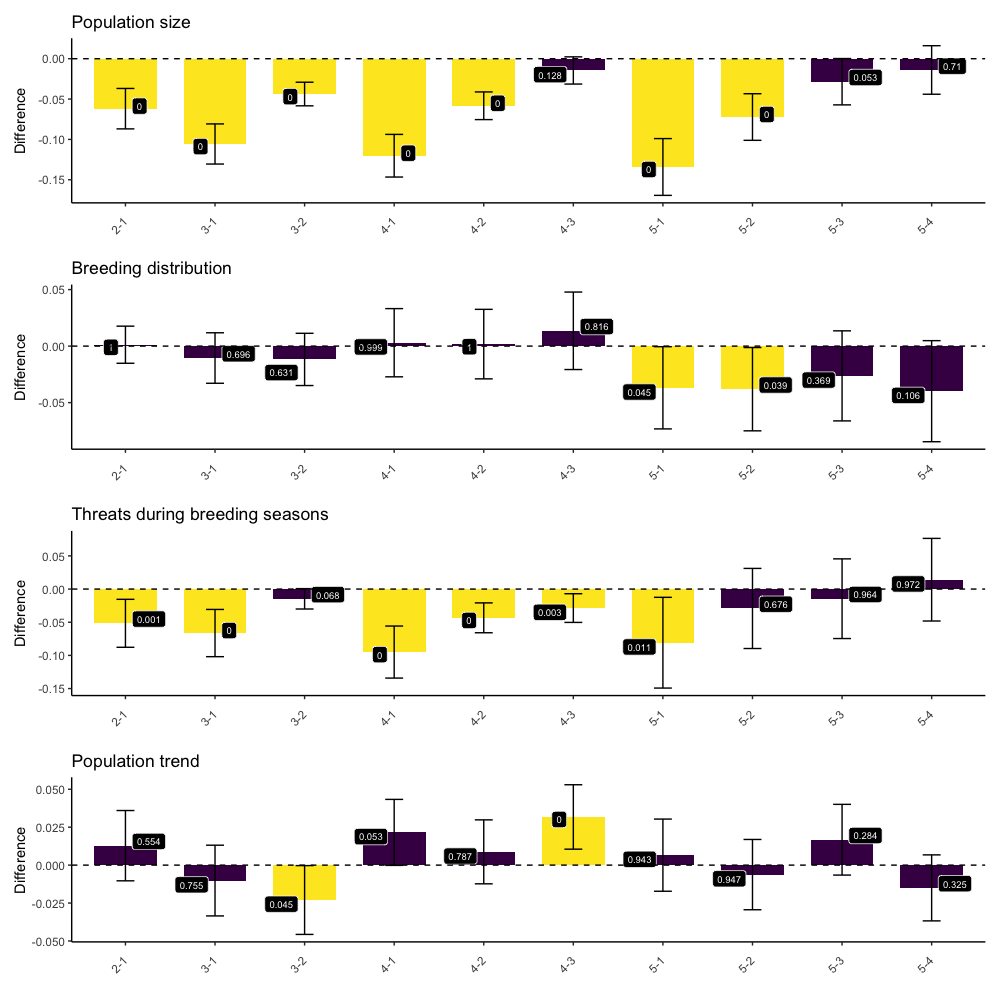
\includegraphics{Figure4.png} \textbf{Figure 4. Continental
vulnerability level of all native continental birds in the United States
and associated domestic cat predation pressure based on the Bird
Conservation Assessment Database.} Each bar in the figure represents the
difference between the means of two levels of the score, ranging from 1
to 5, where 1 indicates the least threatened species and 5 the most
threatened. The bracket accompanying each bar indicates the 95\%
confidence interval based on the Tukey honest significant differences of
the mean difference. The corresponding p-value is provided in white
font.

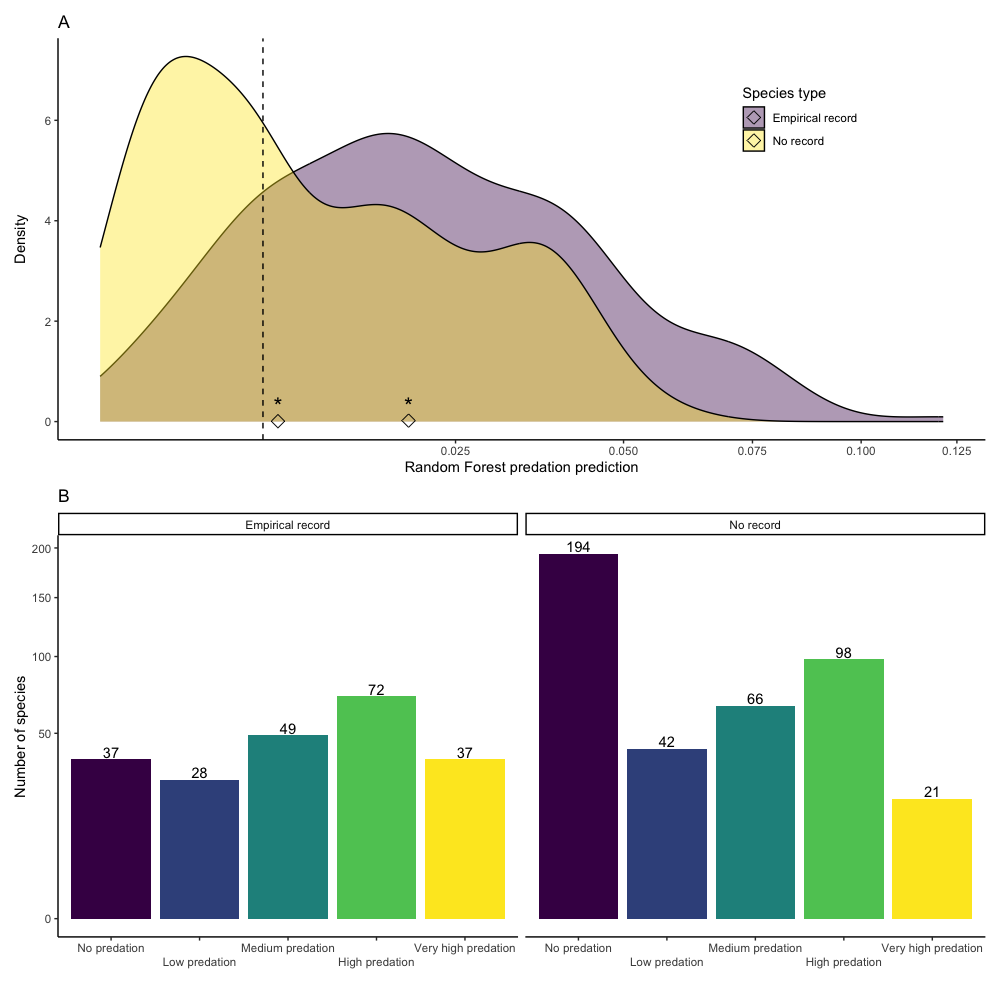
\includegraphics{Figure5.png} \textbf{Figure 5. Comparison of predation
pressure predicted by Random Forest and empirical records of predation
events by domestic cats for all native continental birds in the United
States.} Panel A displays the distribution of species with empirical
records of predation by domestic cats in North America (referred to as
`prey species') and species without records (`non-prey species'). These
distributions are plotted along the values of predation pressure
predicted by the Random Forest regression model. The difference between
the two distributions is evaluated by comparing the median values,
indicated by black diamonds, using a permutation test. The stars above
the diamonds indicate a significant difference at the 5\% level. Panel B
depicts the distribution of species from both groups based on their
predation pressure classifications. Each bar represents the number of
species per classification of predation pressure for species with or
without empirical records of predation by domestic cats in North
America. The numbers above the bars indicate the species count for each
predation pressure classification, thus providing a visual
representation of the distribution patterns for both categories.



\end{document}
